%%%%%%%%%%%%%%%%%%%%%%%%%%%%%%%%%%%%%%%%%
%
% (c) 2022 by Jennifer Laaser
%
% This work is licensed under the Creative Commons Attribution-NonCommercial-ShareAlike 4.0 International License. To view a copy of this license, visit http://creativecommons.org/licenses/by-nc-sa/4.0/ or send a letter to Creative Commons, PO Box 1866, Mountain View, CA 94042, USA.
%
% The current source for these materials is accessible on Github: https://github.com/jlaaser/pogil-polymers
%
%%%%%%%%%%%%%%%%%%%%%%%%%%%%%%%%%%%%%%%%%

\renewcommand{\figpath}{content/polymchem/livingpolyms/anionic-polyms/figs}
\renewcommand{\labelbase}{anionic-polyms}

\begin{activity}{Anionic Polymerizations}

\begin{instructornotes}
	This activity introduces students to concepts related to anionic polymerization.
	
	After completing this activity, students will be able to:
	\begin{enumerate}
		\item Predict the polymer structure formed from given reagents in an anionic polymerization
		\item Explain why (and under what conditions) anionic polymerizations approximate an ideal living polymerization
		\item Explain how anionic polymerization can be used to synthesize block copolymers
	\end{enumerate}
	
	\subsection*{Activity summary:}
	\begin{itemize}
		\item \textbf{Activity type:} Learning Cycle
		\item \textbf{Content goals:} See above
		\item \textbf{Process goals:} %https://pogil.org/uploads/attachments/cj54b5yts006cklx4hh758htf-process-skills-official-pogil-list-2015-original.pdf
			\begin{itemize}
				\item Reading and interpreting reaction mechanisms
				\item Oral and written communication of reasoning
			\end{itemize}
		\item \textbf{Duration:} 45 minutes, including class discussion
		\item \textbf{Instructor preparation required:} none beyond knowledge of relevant content
		\item \textbf{Related textbook chapters:}
			\begin{itemize}
				\item \emph{Polymer Chemistry} (Hiemenz \& Lodge), 2nd ed.: section 4.3
				\item \emph{Introduction to Polymers} (Young \& Lovell), 3rd ed.: section 5.3
			\end{itemize}
		%\item \textbf{Facilitation notes:}
		%	\begin{itemize}
		%		\item \dots
		%	\end{itemize}
	\end{itemize}
	
\end{instructornotes}


\begin{model}[Basics of Anionic Polymerization]
	\label{\labelbase:mdl:anionic}

	Anionic polymerization is a popular method for producing polymers with well-controlled molecular weights.  The initiation and propagation steps of the anionic polymerization of a vinyl-type monomer are outlined below:
	
	\centerline{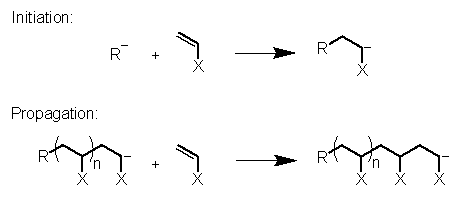
\includegraphics[width=0.7\textwidth]{\figpath/MODEL1_mainscheme}}
	
\end{model}


\begin{ctqs}

	%\question What is the reactive species on the initiator and chain ends in this type of polymerization?
	
	\question Which reagent determines the number of polymer chains formed in this reaction?
	
		\begin{solution}[0.25in]
			The initiator anion, R\textsuperscript{-}
		\end{solution}
	
	\question If the reaction proceeds to 100\% conversion (i.e. 100\% of the monomer is used up in the reaction), how would you expect the degree of polymerization of the resulting polymer to be related to the initiator and monomer concentrations, $[I]_0$ and $[M]_0$?
	
		\begin{solution}[0.5in]
			Number-average degree of polymerization is just number of monomers divided by number of chains.  The number of chains is equal to the number of initiators, so $N_n = \frac{[M]_0}{[I]_0}$
		\end{solution}
	
	\question One initiator that can be used in anionic polymerization is \emph{sec}-butyllithium, shown below:
	 \label{\labelbase:ctq:ps-anionic-prop}
	
	\centerline{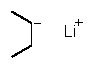
\includegraphics[width=0.15\textwidth]{\figpath/MODEL1_secBuLi}}
	 	
	 	Draw the structure of the propagating chain that would be formed if this reagent were used to initiate anionic polymerization of polystyrene.
	 	
	 	\emph{Note: For the purposes of this question, you can assume that the lithium ion does not participate in the reaction in any way.}
	
		\begin{solution}[1in]
		\studentdisplay{}
		\instructordisplay{\centerline{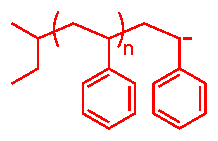
\includegraphics[width=0.3\textwidth]{\figpath/MODEL1_propchain}}}
		\end{solution}
	
	\question Suppose two propagating anions encounter each other in solution, as shown below:
	
	\centerline{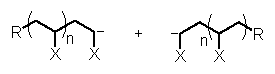
\includegraphics[width=0.4\textwidth]{\figpath/MODEL1_anionterm}}
	
		Do you expect these two anions to be able to react to form inactive (``dead'') polymer chains?  Explain your group's reasoning in 1-2 complete sentences.
	
		\begin{solution}[1.25in]
			No, these two anions should not be able to react to form inactive/dead polymer chains.  Generally, two anions cannot react directly with each other to form a neutral molecule.
		\end{solution}
	
	\question On the basis of your answer to the previous question, do you expect anionic polymerization to meet the criteria required for an ideal, living polymerization?  Explain your group's reasoning in 2-3 complete sentences.
	
		\begin{solution}[1.25in]
			Yes, given this information, anionic polymerization should meet the criteria for a living polymerization, because it proceeds in the absence of termination.
			
			Students do not really have enough information from the model to determine whether it is also an \textit{ideal} polymerization, but generally speaking, if carried out correctly anionic polymerization does indeed qualify because initiation is fast enough that all chains essentially initiate at once, and the chains also all grow at the same rate.  If done well, it is very possible to obtain dispersities of less than 1.05 (or even 1.01) via anionic polymerization.
		\end{solution}

\end{ctqs}

\begin{infobox}

	If the propagating anion encounters a molecule with a labile proton, it will typically be favorable for it to abstract that proton, as shown below:
	
	\centerline{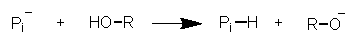
\includegraphics[width=0.6\textwidth]{\figpath/MODEL1_labileproton}}
	
\end{infobox}

\begin{ctqs}
	
	%\question Briefly describe what you would expect to happen to the propagating species in an anionic polymerization if the reaction mixture contained a small amount of water.  In this case, would the reaction still be an ideal, living polymerization?
	
	\question Why might we say that the presence of a species with a labile proton terminates the propagating anionic chain?  Explain your group's reasoning in 1-2 complete sentences.
	
		\begin{solution}[1in]
			When the propagating anion abstracts the proton, the chain is capped with (and ``neutralized'' by) that proton and no longer contains an anionic site that can attack additional monomers.
		\end{solution}
	
	\question If your reaction mixture contained a small amount of water, would you still expect the reaction to qualify as an ideal, living polymerization?  Why or why not?
	
		\begin{solution}[1.25in]
			No, if the reaction mixture contained water, the propagating chains would terminate by abstracting a proton from water.  The polymerization would thus no longer be proceeding in the absence of irreversible termination, and would no longer be living.
		\end{solution}
	
	\question Based on your answer to the previous question, explain, in 1-2 complete sentences, why it is typically critical that the solvent and monomers used in anionic polymerizations are \emph{rigorously} dried before use.
	
		\begin{solution}[1.25in]
			If the solvents and monomers are not rigorously dried before use, they may contain small amounts of water, which will terminate some of the chains and increase the dispersity of the polymer obtained in the polymerization.
		\end{solution}
	
\end{ctqs}

\begin{infobox}

	While \emph{unintentional} introduction of hydroxyl-containing species causes problems with anionic polymerization, \emph{intentional} introduction of a hydroxyl-containing species at the end of the reaction can be a useful way to terminate the polymer in a well-controlled way.  For example, anionic polymerizations are often terminated by addition of a small amount of methanol.

\end{infobox}

\begin{ctqs}

	\question Predict the structure of the polymer that you would obtain if you terminated the propagating anionic chain you drew in CTQ \ref{\labelbase:ctq:ps-anionic-prop} by adding methanol at the end of the reaction.
	
		\begin{solution}[2in]
		\studentdisplay{}
		\instructordisplay{\centerline{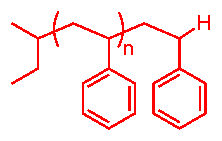
\includegraphics[width=0.3\textwidth]{\figpath/MODEL1_terminated}}}
		\end{solution}

	%\question introduce idea that other types of monomers can also go by anionic -> show propagation step of ethylene oxide (mention that it is a ring-opening polym, which we we will explore more later) and ask them to predict product when RO- polyms ethylene oxide w/methanol to terminate
		
\end{ctqs}


\clearpage
\begin{model}[Polymerization of Ethylene Oxide]
	\label{\labelbase:mdl:anionicEO}

	Although anionic polymerization is shown using a vinyl type monomer in Model \ref{\labelbase:mdl:anionic}, above, it can be used to polymerize a number of other types of monomers, as well.
	
	One common monomer polymerized by anionic polymerization is ethylene oxide.  Polymerization of this monomer proceeds as shown below:
	
	\centerline{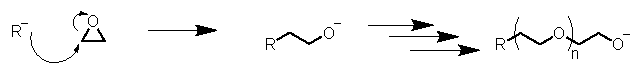
\includegraphics[width=0.9\textwidth]{\figpath/MODEL2_EOprop}}

\end{model}

\begin{ctqs}
	
	\question Why do you think polymerization of ethylene oxide is referred to as a ``ring-opening'' polymerization?  Explain your group's reasoning in 1-2 complete sentences.
	
		\begin{solution}[1in]
			Polymerization of ethylene oxide is considered a ring-opening polymerization because the monomer (ethylene oxide) is a 3-membered ring, and it is opened up to form a linear segment of the polymer backbone (containing 3 bonds).
		\end{solution}
	
	\question Predict the structure of the polymer that you would obtain if you used the propagating chain from CTQ \ref{\labelbase:ctq:ps-anionic-prop} as the initiator for polymerization of ethylene oxide, and if you terminated the reaction with methanol after all of the ethylene oxide was used up.
	
		\begin{solution}[1.75in]
		\studentdisplay{}
		\instructordisplay{
			\centerline{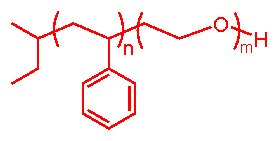
\includegraphics[width=0.25\textwidth]{\figpath/MODEL2_PSbPEO}}
			
			NOTE: practically speaking, the PS macroinitiator from CTQ \ref{\labelbase:ctq:ps-anionic-prop} can't be used to directly initiate polymerization of PEO, because PEO does not propagate well with Li\textsuperscript{+} counterions.  Instead, only a single EO unit adds. The polymer must be terminated with MeOH and then re-initiated with a K\textsuperscript{+} counterion (using e.g. potassium naphthalenide) to successfully synthesize the PEO block.  See DOI:10.1021/la504605e for an example.
		}
		\end{solution}
	
	\question Propose a complete name for the polymer you drew in the previous question.  Make sure the name you propose clearly specifies the identity (or identities) of the constituent polymers, whether the polymer is a homopolymer, copolymer, or terpolymer, and what its general chain architecture and sequence type are. 
	
		\begin{solution}[1in]
			poly(styrene)-\emph{block}-poly(ethylene oxide)
			
			(a block copolymer)
		\end{solution}
		
	\question Critique or defend the following statement in 2-3 complete sentences:
	
		\emph{``The living nature of anionic polymerizations makes them a useful way to synthesize block copolymers.''}
		
		\begin{solution}[1.5in]
			This statement is generally true.  Anionic polymerization lends itself well to synthesis of block copolymers because it (1) typically produces narrow dispersity polymers with a reactive site retained on nearly 100\% of the chains, allowing uniform addition of each successive block, and (2) typically proceeds to 100\% or nearly 100\% conversion of monomers, meaning that the next block can be synthesized without having to isolate or purify the previous block.
		\end{solution}
	
\end{ctqs}


\begin{exercises}

%	\exercise exercise re. the cation

	\exercise The initiation reaction in anionic polymerization can be written (simply) as %note: this question should probably eventaully just get turned into Model 3, but I'm going to leave it in the Exercises for now.
		\begin{equation*}
			R^- + M \ce{->} RM^-
		\end{equation*}
		
		\begin{enumerate}
			\item For this reaction to be favorable, which anion must be more stable, R$^-$ or M$^-$?
			
				\begin{solution}\instructordisplay{
					M$^-$ must be more stable.
				}\end{solution}
				
			\item One way to gauge anion stability is to look at the pKa of the conjugate acid.  Recall that the pKa for the following reaction
					\begin{equation*}
						RH \ce{<=>} R^- + H^+
					\end{equation*}
				is given by 
					\begin{equation*}
						pKa = -\log_{10} K_a
					\end{equation*}
				where
					\begin{equation*}
						K_a = \frac{[R^-][H^+]}{RH}
					\end{equation*}
					
					Based on this information, does a higher pKa indicate that the anion $R^-$ is more or less stable?  Explain your reasoning in 1-2 complete sentences.
					
				\begin{solution}\instructordisplay{
					A higher pKa indicates that the anion R$^-$ is \emph{less} stable.  A higher pKa means that the equilibrium constant $K_a$ is smaller, which in turn means that the protonated species RH is more favored.  By contrast, a lower pKa means that the equilibrium constant $K_a$ is larger, which means that it is more favorable to form the anionic species R$^-$ (which we in turn assume means that the anionic species R$^-$ is more stable).
				}\end{solution}
				
			\item Look up the pKa's of butane and toluene.  Based on these pKa's, do you expect \emph{n}-butyllithium to be an effective initiator for anionic polymerization of styrene?
			
				\begin{solution}\instructordisplay{
					The pKa of the methyl group on butane is approximately 50-60, and that of the methyl group in toluene (which is a good approximation for the conjugate acid of the styryl anion) is about 40.  This means that we \emph{should} be able to initiate polymerization of styrene using n-butyllithium, because the propagating anion formed upon the first monomer addition will be more stable than that of the initiator.
				}\end{solution}
				
			
			\item Now, suppose you want to synthesize a block copolymer of polystyrene and poly(methyl methacrylate) by directly adding the second monomer to the reaction mixture after polymerization of the first block is complete.  Which order would you need to synthesize the two blocks in, and why?  Justify your reasoning in 2-3 complete sentences.
			
				\emph{Hint: you will probably find it helpful to look up the pKa of ethyl acetate.}.
			
				\begin{solution}\instructordisplay{
					You need to polymerize the styrene block first.  Ethyl acetate (which, again, is a good approximation for the conjugate acid of the propagating species in polymerization of MMA) has a pKa of about 25.  This is lower than that  of toluene (our reference for polymerization of styrene), indicating that the propagating anion formed in polymerization of MMA is more stable than that formed in polymerization of styrene.  Thus, a propagating styryl anion will be able to initiate polymerization of MMA, but not the other way around.
				}\end{solution}
				
		\end{enumerate}

	\exercise Nominally, the polymerization rate in an anionic polymerization obeys
		\begin{equation*}
			R_p = -\frac{d\text{[M]}}{dt} = k_p\text{[M][P}^-\text{]}
		\end{equation*}
		where [M] and [P\textsuperscript{-}] are the concentrations of monomer and anionic chain ends, respectively, and $k_p$ is the propagation rate constant.
		
		In most nonpolar solvents, however, the highly polar ionic groups on the ends of the polymer chains often cluster together, and these clusters (or aggregates) exist in equilibrium with the free chains, as show below:
			\begin{equation*}
				\underbrace{(P^-)_n}_{\text{cluster/aggregate}} \ce{<<=>} \underbrace{n\,\,P^-}_{\text{free chains}}
			\end{equation*}
		When this occurs, only the free chains are able to engage in propagation reactions, and [P\textsuperscript{-}] in the above expression should be replaced by [P\textsuperscript{-}]\textsubscript{free}.
		
		Based on this information, do the following:
		\begin{enumerate}
			\item Write an expression for the equilibrium constant $K_{dis}$ representing dissociation of the cluster into $n$ free chains, in terms of the concentration of clusters, [(P\textsuperscript{-})\textsubscript{n}], and the concentration of free chains, [P\textsuperscript{-}]\textsubscript{free}.
				
				\begin{solution}\instructordisplay{
					\begin{equation*}
						K_{dis} = \frac{\text{[P}^-\text{]}^n_{\text{free}}}{\text{[(P}^-\text{)}_n\text{]}}
					\end{equation*}
				}\end{solution}
				
			\item Solve for the concentration of free chains and use your result to obtain an expression for $R_p$ in terms of $K_{dis}$ and the concentration of clusters.
				
				\begin{solution}\instructordisplay{
					Solving for the concentration of free chains, we find
					\begin{equation*}
						\text{[P}^-\text{]}_{\text{free}} = \left(K_{dis}\text{[(P}^-\text{)}_n\text{]}\right)^{1/n}
					\end{equation*}
					Substituting this result into the expression for $R_p$, we obtain
					\begin{equation*}
						R_p = k_p\text{[M]}\left(K_{dis}\text{[(P}^-\text{)}_n\text{]}\right)^{1/n}
					\end{equation*}
				}\end{solution}
				
			\item Explain why it might be reasonable to approximate the concentration of clusters as [(P\textsuperscript{-})\textsubscript{n}]$\approx \frac{1}{n}$[P\textsuperscript{-}], where [P\textsuperscript{-}] is the \emph{total} number of anionic chains in the system (whether in a cluster or not).  Once you have convinced yourself this is reasonable, use it to rewrite your expression from the previous part to obtain an expression for $R_p$ in terms of $K_{dis}$ and the total concentration of anionic chains.
				
				\begin{solution}\instructordisplay{
					If the solvent conditions strongly favor clustering of the ions, then most of the chains will be in clusters.  As a result, the total concentration of chains is essentially the number of chains per cluster times the number of clusters, yielding [P\textsuperscript{-}]$=n$[(P\textsuperscript{-})\textsubscript{n}], or [(P\textsuperscript{-})\textsubscript{n}]$\approx \frac{1}{n}$[P\textsuperscript{-}] as desired.
					
					Substituting this in to the expression for $R_p$, we obtain
					\begin{equation*}
						R_p = k_p\text{[M]}\left(K_{dis} \frac{1}{n}[P\textsuperscript{-}]\right)^{1/n}
					\end{equation*}
					With a bit of rearrangement, we can also write this as
					\begin{equation*}
						R_p = k_{app} \text{[M]} [P\textsuperscript{-}]^{1/n}
					\end{equation*}
					where $k_{app} = k_p\left(\frac{K_{dis}}{n}\right)^{1/n}$
				}\end{solution}
				
			\item Finally, use the results of your analysis to critique or defend the following statement in 2-3 complete sentences:
			
			\emph{``Anionic polymerization is typically much faster in nonpolar solvents than it is in polar solvents.''}
				
				\begin{solution}\instructordisplay{
					This statement is \emph{false}.  In nonpolar solvents, clusters do form (so $n > 1$), and the equilibrium constant favors clusters over free chains ($K_{dis}< 1$).  As a result, not only is $k_{app}<k_p$, but also $[P\textsuperscript{-}]^{1/n} < [P\textsuperscript{-}]$.  Both of these effects significantly slow the reaction rate relative to what would be observed in the absence of ion clustering.
					
					Note that this change in the kinetics can also have other effects, such as allowing time for monomers at the chain end to isomerize before the next monomer is added, which can affect \emph{cis}-\emph{trans} ratios in (for example) polyisoprene; for discussion of this point, see Section 4.3 of \emph{Polymer Chemistry} by Hiemenz \& Lodge.
				}\end{solution}
				
		\end{enumerate}

%	\exercise question re. expected behavior of a PS-b-PEO block copolymer if dissolved in water, in limit that PS length > EO, PS = EO, PS < EO
	
\end{exercises}


%\begin{problems}
%
%	\problem First exercise
%	\problem Second exercise
%	
%\end{problems}


	
\end{activity}